\chapter{Lecture 21 - Monte Carlo Methods for Numeric Integration}
\label{ch:lec21n}
\section{Objectives}
The objectives of this lecture are to:
\begin{itemize}
\item Describe two simple algorithms for carrying out numerical integration with the Monte Carlo method.
\item Provide some suggestions as to when different numerical integration algorithms are appropriate
\end{itemize}
\setcounter{lstannotation}{0}
\section{Introduction}
Most every integration problem that you are likely to encounter in your time as an engineer can be solved by one of the methods described in the last two lectures---possibly with some extensions or modification.\sidenote{Notably, we have not yet discussed integration over more than one dimension and we have side-stepped issues such as infinite domains of ntegration or integrals over intervals in which the integrand has one or more singularities.  We have ways of dealing with these problems that have been omitted in sympathy for your endurance.  We walk before we run.}  Still, in the spirit of skinning the cat in as many ways as we can, and to help us acknowledge that some problems can be approached from many different ways, in this lecture we introduce Monte Carlo quadrature.

Monte Carlo quadrature involvs solving the integral at hand by changing the problem into a game of chance.  There are several textbooks that introduce this method along with Monte Carlo methods for solving a variety of other problems.For an engineer-friendly introduction, see chapter 42 and 43 of the excellent book by Farlow.\cite{farlow1993partial}.  For a more in-depth treatment that includes important applications for nuclear engineers, see the text by Dunn.\cite{dunn2022exploring}

\section{Hit or Miss Algorithm}
The ``Hit or Miss'' algorithm is probably the simplest example of a Monte Carlo method for quadrature.  The algorithm is as follows:
\begin{enumerate}
\item Establish a simple area---a ``bounding box''---that bounds the function of interest.
\item Take uniform random samples from points within the bounding box.
\item Determine the fraction of the random samples that fall ``under'' the function to be integrated.
\item Multiply that fraction by the area of the bounding box; this is your Monte Carlo estimate of the integral.
\end{enumerate}

\vspace{0.25cm}

\noindent\textbf{Example:} Us the hit-or-miss method to estimate the following integral:
\begin{equation*}
\int_{-3}^{3} e^{-x^2} \ dx
\end{equation*}

\begin{marginfigure}
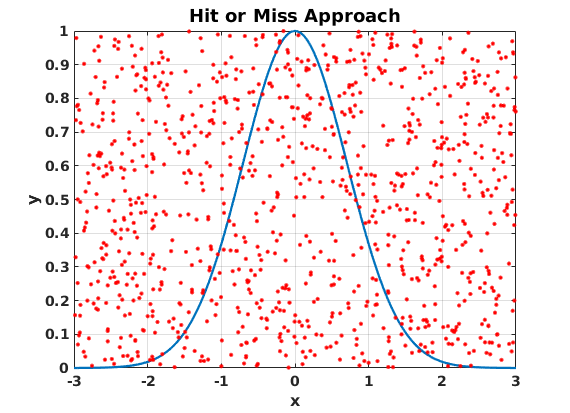
\includegraphics{lec21n-hit-or-miss-schematic.png}
\caption{Sample of 1000 uniformly distributed random points from withn the box $[-3,3]\times[0,1]$.}
\label{fig:lec21n-hit-or-miss-schematic}
\end{marginfigure}

\begin{enumerate}
\item The function has a maximum value at $x=0$: $e^{-0^2} = 1$.  A logical bounding box would therefore be: $x \in [-3,3]$, $y \in [0,1]$.  The area of the bounding box is 6.

\item Figure \ref{fig:lec21n-hit-or-miss-schematic} shows a sample of 1000 uniformly distributed points from within this bounding box.

\item Use MATLAB to determine if $y_{\text{sample}} < f(x_{\text{sample}})$.  If it is, then the point lies ``under'' the curve to be integrated.  Do this for each sample point and calculate the total fraction under the curve.

\item Multiply the fraction by 6 (area of the bounding box) to obtain the estimated integral.
\end{enumerate}

MATLAB code to carry out such a calculation is shown in the listing below.

\begin{lstlisting}[style=myMatlab,name=lec21-ex1]
clear
clc
close all

%% Parameters
f = @(x) exp(-x.^2);
a = -3; b = 3;
fMax = 1; fMin = 0;
N = 1e6; % number of samples

%%

% Compute area of bounding box
Abox = (b-a)*(fMax-fMin); 

% Get N uniformly distributed random numbers
% from within the bounding box
x_s = a + (b-a)*rand(N,1);
y_s = fMin + (fMax-fMin)*rand(N,1);

% Determine how many points fall under f(x)
hit = sum(y_s <= f(x_s));

% Calculate ratio of "Hits"
hit_frac = hit/N;

% Estimated integral
MCInt = hit_frac*Abox;

fprintf('Hit or Miss estimated integral = %g \n',MCInt);
\end{lstlisting}

\begin{marginfigure}
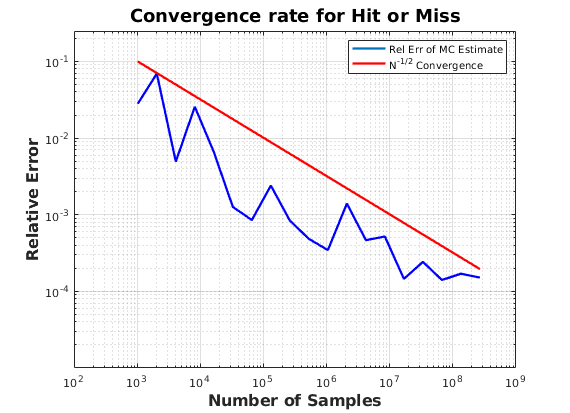
\includegraphics{lec21n-hom-convergence.png}
\caption{Convergence behavior of the Monte Carlo numeric integration algorithm.}
\label{fig:lec21n-hom-convergence}
\end{marginfigure}

Naturally, we expect that our approximation of the integral will improve if we take more random samples.  This turns out to be true and the convergence behavior is illustrated in Figure \ref{fig:lec21n-hom-convergence}.  Notice that the rate of convergence is quite slow with ``half''-order convergence; to reduce error by a factor of 10, you need to do 100 times as much work. 

\section{Mean Value Algorithm}
One simple optimization will allow us to cut the amount of work we need to do in half.  We know from calculus that there is a relationship between the definite integral of a function and its mean value over the interval $x \in [a,b]$.

\begin{equation}
f_{\text{AVG}} = \frac{1}{b-a}\int_{a}^{b} f(x) \ dx
\label{eq:lec21n-mean-value-thm}
\end{equation}

\noindent We can turn this into a Monte Carlo algorithm by turning the equation around:
\begin{enumerate}
\item Sample $f(x)$ uniformly at $N$ random locations within the interval $[a,b]$
\item Approximate $f_{\text{AVG}}$ as:
\begin{align*}
f_{\text{AVG}} &= \frac{1}{N}\sum\limits_{i=1}^{N}f(x_i) \\
\int_{a}^{b} f(x) \ dx &\approx \frac{b-a}{N}\sum\limits_{i=1}^{N}f(x_i)
\end{align*}
\end{enumerate}

\noindent The nice thing about the Mean Value algorithm is that it requires only half as many random numbers as the Hit or Miss algorithm so it runs roughly twice as fast.  The bad part is that it does nothing to improve upon the slow rate of convergence of the Monte Carlo methods.  

\section{Good Features of Monte Carlo Integration}
For simple one-dimensional integrals of smooth ``well-behaved'' functions, Monte Carlo is not competitive with the various Newton-Cotes or Gaussian quadrature schemes discussed in previous lectures.  Monte Carlo methods do, however, have some very nice properties which are enough to justify having them in your tool-bag of quadrature methods.

\begin{marginfigure}
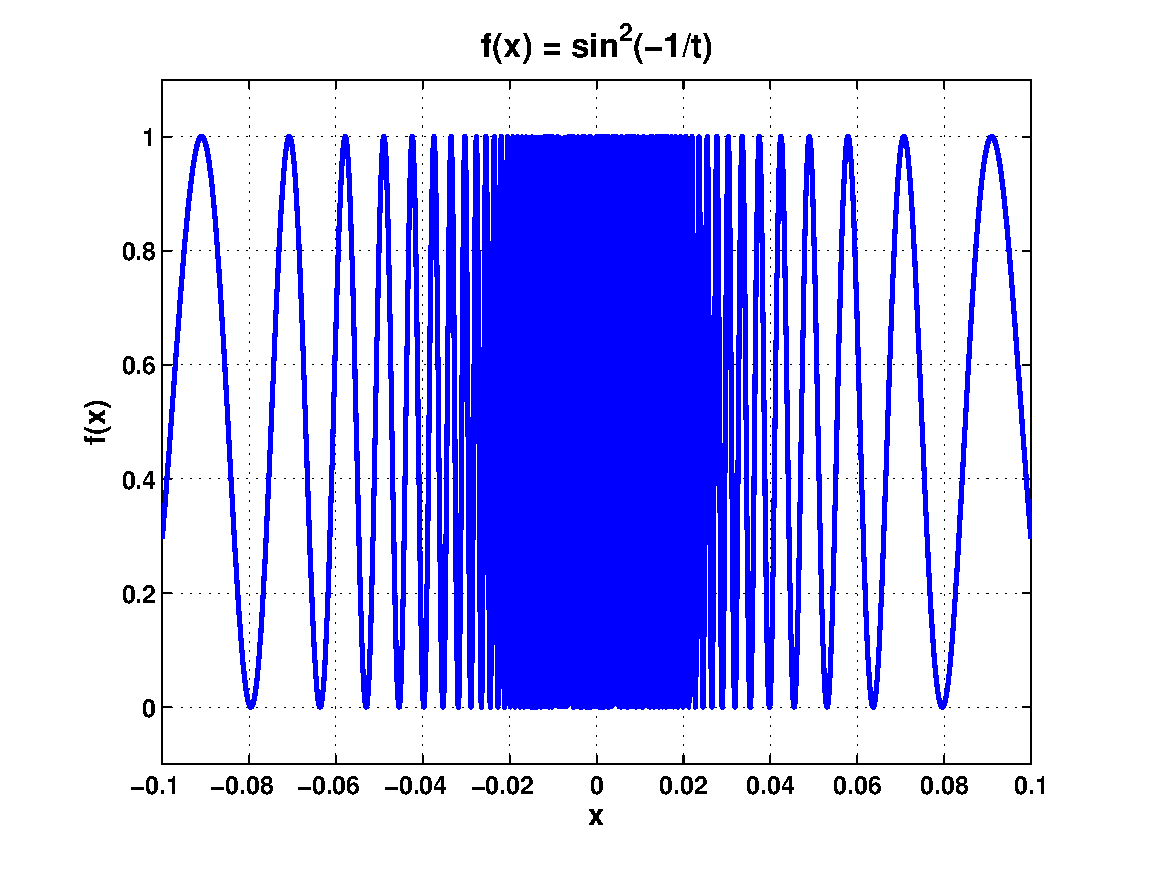
\includegraphics{lec21n-wiggly.eps}
\caption{An example of a function that Newton-Cotes and Gauss quadrature do not integrate well.}
\label{fig:lec21n-wiggly}
\end{marginfigure}


\begin{enumerate}
\item \textbf{Monte Carlo quadrature works well for non-smooth, non-``well-behaved'' functions.}  Consider the ``wiggly'' function shown in Equation \ref{eq:lec21n-wiggly} and plotted in Figure \ref{fig:lec21n-wiggly}.    
\begin{equation}
f(t) = \sin^2{\left(\frac{1}{t} \right)}
\label{eq:lec21n-wiggly}
\end{equation}
Newton-Cotes and Gaussian quadrature algorithms perform very poorly on functions like this since the spacing of sample points must be very tight if the oscillatory behavior of the function is to be captured.  The accuracy of Monte Carlo methods, on the other hand, do not depend on being able to construct a suitable approximation of the integrand.  

\item \textbf{The rate of convergence is independent of the dimensions of integration.} We have not discussed 2D, 3D or more generally N-dimensional integration in any of the last three lectures.  Still, these are important problems both for you as well as your friends in other disciplines.  For Monte Carlo quadrature, the integraation error is always proportional to $\sfrac{1}{\sqrt{n}}$.  The convergence of Newton-Cotes or Gaussian quadrature is actually dependent on the dimensionality.  For example, the error the trapezoidal rule is actually proportional to $\sfrac{1}{\left(n^{\sfrac{2}{D}}\right)}$ where $D$ is the number of spatial dimensions.  This ``curse of dimensionality'' is especially important, for example, for certain problems of statistical physics where the integrations must be performed over billions of dimensions; each ``dimension'' representing an interaction between a pair of bodies.  In this case, use of any method \emph{other} than Monte Carlo is a practical impossibility.

\item \textbf{Monte Carlo methods are very easy to parallelize.} This is important in a day and age when nearly every computer has multiple cores.  Devising algorithms that can efficiently use large parallel computers is a difficult task.\sidenote{And, sadly, a task that is not addressed in this text.}  Monte Carlo methods fit well in a computational ecosystem adaptable to supercomputers.

\end{enumerate}

\section{Which Method to Use?}
Given the variety of integraion method discussed over the last three lectures, you might be wondering why we do not simply pick the best one and always use it.  The reason, of course, is that which one is best depends on your problem.  

\vspace{0.1cm}

\noindent\textbf{Guidelines:}
\begin{enumerate}
\item For integrations where you must sample the functions at regular intervals---e.g. if the function you are integrating is known to you only through the data provided by lab instrumentation---then the trapezoidal or Simpson's rule may be the only choices that are reasonable.  Pick one.

\item For low-dimensional integrations where the function is reasonably smooth and you can sample the function in any place you wish, use Gauss quadrature.  Finite element methods that we will discuss in future lectures use variations of Gauss quadrature extensively because they achieve high accuracy with relatively little work.

\item For high-dimension and/or highly non-smooth functions that you can sample in any place you wish, use Monte Carlo methods.  
\end{enumerate}
